%!TEX root = ./main.tex
Retomamos la definición dada en la sección 2.4 del grupo de trenzas puro, en primera instancia desde un punto de vista netamente algebraico si bien no es imposible resulta difícil pensar en que elementos de $B_n$ pertenecen al kernel de la proyección natural al grupo simétrico. Aqui es donde entra en juego la visualización de los generadores de $B_n$ como cruces en nuestros diagramas de trenzas.

Dada una trenza $\beta$, si tomamos su representación por $D$ la podemos escribir como $\beta=\beta(D)=\sigma_{i_1}^{\varepsilon_1}\dots\sigma_{i_k}^{\varepsilon_k},$ luego por la proyeccion tenemos que
$$\pi(\beta)=(i_1\,i_1+1)\cdots(i_k\, i_k+1).$$
Note que para que este sea la identidad en $S_n$ debería de fijar a todos los elementos de $\{1,2,\ldots,n\}$, esto se traduce a que una cuerda con punto inicial $(i,0)$ debe terminar en el punto $(i,1)$. Así una trenza pura en $n$ cuerdas serán aquellas trenzas con permutacion subyacente $(1,2,\ldots,n)$, pero en particular hay una de estas trenzas que es de gran importancia
\begin{definition}
    Definimos $A_{i,j}\in P_n$ como la trenza dada por
    $$A_{i,j}:=\sigma_{j-1}\sigma_{j-2}\cdots\sigma_{i+1}\sigma_i^2\sigma_{i+1}^{-1}\cdots\sigma_{j-2}^{-1}\sigma_{j-1}^{-1}.$$ 
    Para $1\leq i<j\leq n$
\end{definition}
Antes de ver la ilustración general de esta trenza veamos un ejemplo pequeño construido desde la concatenación de diagramas
\begin{eg}
    Consideremos $A_{2,5}\in P_5\leq B_5$, en términos de generadores seria $\sigma_4\sigma_3\sigma_2^2\sigma_3^{-1}\sigma_4^{-1}$, los diagramas de cada una de estas concatenados seria el siguiente
    \begin{center}
        

\tikzset{every picture/.style={line width=0.75pt}} %set default line width to 0.75pt        

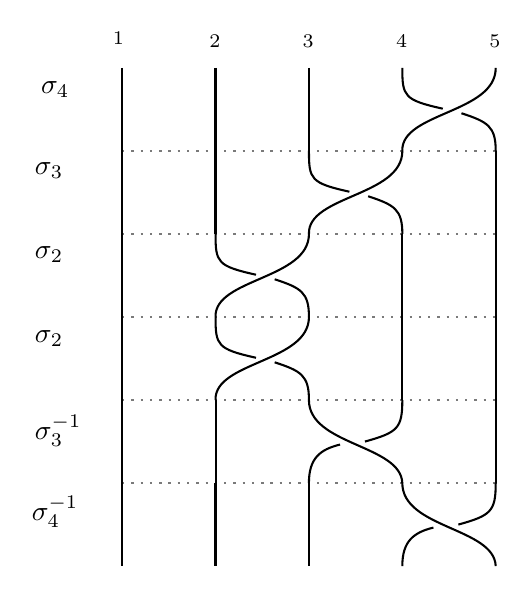
\begin{tikzpicture}[x=0.75pt,y=0.75pt,yscale=-1.5,xscale=1.5]
%uncomment if require: \path (0,877); %set diagram left start at 0, and has height of 877

%Straight Lines [id:da4528615870084317] 
\draw    (110,30) -- (110,56.67) ;
%Straight Lines [id:da9766817859581656] 
\draw    (140,30) -- (140,56.67) ;
%Straight Lines [id:da5434211752169944] 
\draw    (170,30) -- (170,56.67) ;
%Curve Lines [id:da18588234162034845] 
\draw    (230,30) .. controls (230,44.55) and (199.5,44.3) .. (200,56.67) ;
%Curve Lines [id:da6457986192066467] 
\draw    (200,30) .. controls (200,39.09) and (200.5,40.3) .. (213,43.09) ;
%Curve Lines [id:da3965842064327222] 
\draw    (230,56.67) .. controls (230,48.79) and (227.5,47.33) .. (219,44.55) ;
%Straight Lines [id:da050847895402120535] 
\draw    (110,56.67) -- (110,83.33) ;
%Straight Lines [id:da16482821514498391] 
\draw    (140,56.67) -- (140,83.33) ;
%Straight Lines [id:da605256407413367] 
\draw    (230,56.67) -- (230,83.33) ;
%Curve Lines [id:da772060448954358] 
\draw    (200.01,56.67) .. controls (200.01,71.21) and (169.51,70.97) .. (170.01,83.33) ;
%Curve Lines [id:da7499936673128771] 
\draw    (170.01,56.67) .. controls (170.01,65.76) and (170.51,66.97) .. (183.01,69.76) ;
%Curve Lines [id:da3693559341271877] 
\draw    (200.01,83.33) .. controls (200.01,75.45) and (197.51,74) .. (189.01,71.21) ;
%Straight Lines [id:da7202577392744585] 
\draw    (110,83.33) -- (110,110) ;
%Straight Lines [id:da20458946078006213] 
\draw    (200,83.33) -- (200,110) ;
%Straight Lines [id:da8667257213324755] 
\draw    (230,83.33) -- (230,110) ;
%Curve Lines [id:da998274813494859] 
\draw    (170.01,83.33) .. controls (170.01,97.88) and (139.51,97.64) .. (140.01,110) ;
%Curve Lines [id:da6854237975070604] 
\draw    (140.01,83.33) .. controls (140.01,92.42) and (140.51,93.64) .. (153.01,96.42) ;
%Curve Lines [id:da5297642757206432] 
\draw    (170.01,110) .. controls (170.01,102.12) and (167.51,100.67) .. (159.01,97.88) ;
%Straight Lines [id:da9017527301032908] 
\draw    (110,110) -- (110,136.67) ;
%Straight Lines [id:da4955920643850338] 
\draw    (200,110) -- (200,136.67) ;
%Straight Lines [id:da11538535615536005] 
\draw    (230,110) -- (230,136.67) ;
%Curve Lines [id:da37868154219095895] 
\draw    (170.01,110) .. controls (170.01,124.55) and (139.51,124.3) .. (140.01,136.67) ;
%Curve Lines [id:da23742488108016713] 
\draw    (140.01,110) .. controls (140.01,119.09) and (140.51,120.3) .. (153.01,123.09) ;
%Curve Lines [id:da3728771224894599] 
\draw    (170.01,136.67) .. controls (170.01,128.79) and (167.51,127.33) .. (159.01,124.55) ;
%Straight Lines [id:da28473280471632967] 
\draw    (110,136.67) -- (110,163.33) ;
%Straight Lines [id:da16013179953831969] 
\draw    (140.01,136.67) -- (140.01,163.33) ;
%Straight Lines [id:da7657182980846589] 
\draw    (230,136.67) -- (230,163.33) ;
%Curve Lines [id:da8935775795135815] 
\draw    (170,136.67) .. controls (170,151.21) and (199.5,150.97) .. (200,163.33) ;
%Curve Lines [id:da21945978370974606] 
\draw    (200,136.67) .. controls (200,145.76) and (198.5,147.09) .. (188,150) ;
%Curve Lines [id:da2737490660420109] 
\draw    (170,163.33) .. controls (170,155.45) and (173.5,152.55) .. (180,150.97) ;
%Straight Lines [id:da6340007343413002] 
\draw    (110,163.33) -- (110,190) ;
%Straight Lines [id:da002912950705584616] 
\draw    (140,163.33) -- (140,190) ;
%Straight Lines [id:da9249670869790916] 
\draw    (170,163.33) -- (170,190) ;
%Curve Lines [id:da9873495179759113] 
\draw    (200,163.33) .. controls (200,177.88) and (229.5,177.64) .. (230,190) ;
%Curve Lines [id:da6103083548177296] 
\draw    (230,163.33) .. controls (230,172.42) and (228.5,173.76) .. (218,176.67) ;
%Curve Lines [id:da33245303756177] 
\draw    (200,190) .. controls (200,182.12) and (203.5,179.21) .. (210,177.64) ;
%Straight Lines [id:da6510392317653134] 
\draw [color={rgb, 255:red, 0; green, 0; blue, 0 }  ,draw opacity=0.52 ] [dash pattern={on 0.84pt off 2.51pt}]  (110,56.67) -- (230,56.67) ;
%Straight Lines [id:da16081794164754604] 
\draw [color={rgb, 255:red, 0; green, 0; blue, 0 }  ,draw opacity=0.52 ] [dash pattern={on 0.84pt off 2.51pt}]  (110,83.33) -- (230,83.33) ;
%Straight Lines [id:da3942374220673036] 
\draw [color={rgb, 255:red, 0; green, 0; blue, 0 }  ,draw opacity=0.52 ] [dash pattern={on 0.84pt off 2.51pt}]  (110.01,110) -- (230.01,110) ;
%Straight Lines [id:da5126873997037857] 
\draw [color={rgb, 255:red, 0; green, 0; blue, 0 }  ,draw opacity=0.52 ] [dash pattern={on 0.84pt off 2.51pt}]  (110.01,136.67) -- (230.01,136.67) ;
%Straight Lines [id:da5715606626525153] 
\draw [color={rgb, 255:red, 0; green, 0; blue, 0 }  ,draw opacity=0.52 ] [dash pattern={on 0.84pt off 2.51pt}]  (110,163.33) -- (230,163.33) ;

% Text Node
\draw (106,17.4) node [anchor=north west][inner sep=0.75pt]  [font=\scriptsize]  {$1$};
% Text Node
\draw (83,33.4) node [anchor=north west][inner sep=0.75pt]    {$\sigma _{4}$};
% Text Node
\draw (81,59.4) node [anchor=north west][inner sep=0.75pt]    {$\sigma _{3}$};
% Text Node
\draw (81,86.4) node [anchor=north west][inner sep=0.75pt]    {$\sigma _{2}$};
% Text Node
\draw (81,113.4) node [anchor=north west][inner sep=0.75pt]    {$\sigma _{2}$};
% Text Node
\draw (81,140.4) node [anchor=north west][inner sep=0.75pt]    {$\sigma _{3}^{-1}$};
% Text Node
\draw (80,166.4) node [anchor=north west][inner sep=0.75pt]    {$\sigma _{4}^{-1}$};
% Text Node
\draw (137,18.4) node [anchor=north west][inner sep=0.75pt]  [font=\scriptsize]  {$2$};
% Text Node
\draw (167,18.4) node [anchor=north west][inner sep=0.75pt]  [font=\scriptsize]  {$3$};
% Text Node
\draw (197,18.4) node [anchor=north west][inner sep=0.75pt]  [font=\scriptsize]  {$4$};
% Text Node
\draw (227,18.4) node [anchor=north west][inner sep=0.75pt]  [font=\scriptsize]  {$5$};


\end{tikzpicture}


    \end{center}
    Note en esencia la cuerda que empieza en el punto $(5,0)$ pasa por encima de todas salvo de la que empieza en $(1,0)$, gira al rededor de la que empieza en $(2,0)$ y luego vuelve a pasar por encima en el camino de vuelta. Así por medio de una isotopia que tense las cuerdas obtenemos el siguiente diagrama
    \begin{center}
        

\tikzset{every picture/.style={line width=0.75pt}} %set default line width to 0.75pt        

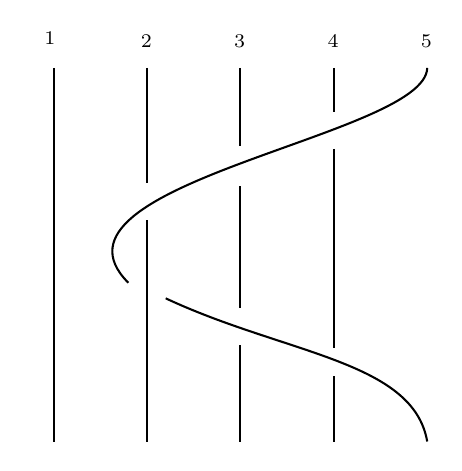
\begin{tikzpicture}[x=0.75pt,y=0.75pt,yscale=-1.5,xscale=1.5]
%uncomment if require: \path (0,877); %set diagram left start at 0, and has height of 877

%Straight Lines [id:da45747682112445587] 
\draw    (110,30) -- (110,150) ;
%Curve Lines [id:da780036391620541] 
\draw    (230,30) .. controls (229.5,52) and (102,67) .. (134,99) ;
%Straight Lines [id:da7231034545363801] 
\draw    (140,30) -- (140,67) ;
%Straight Lines [id:da42500416943536923] 
\draw    (140,79) -- (140,150) ;
%Curve Lines [id:da4654984332204606] 
\draw    (146,104) .. controls (184.5,122) and (225.5,124) .. (230,150) ;
%Straight Lines [id:da9660591521671449] 
\draw    (170,30) -- (170,55) ;
%Straight Lines [id:da38384623850853183] 
\draw    (170,68) -- (170,107) ;
%Straight Lines [id:da7201739522652382] 
\draw    (170,119) -- (170,150) ;
%Straight Lines [id:da2578634464595936] 
\draw    (200,56) -- (200,120) ;
%Straight Lines [id:da21734786864923916] 
\draw    (200,30) -- (200,44) ;
%Straight Lines [id:da1231057225472203] 
\draw    (200,129) -- (200,150) ;

% Text Node
\draw (106,17.4) node [anchor=north west][inner sep=0.75pt]  [font=\scriptsize]  {$1$};
% Text Node
\draw (137,18.4) node [anchor=north west][inner sep=0.75pt]  [font=\scriptsize]  {$2$};
% Text Node
\draw (167,18.4) node [anchor=north west][inner sep=0.75pt]  [font=\scriptsize]  {$3$};
% Text Node
\draw (197,18.4) node [anchor=north west][inner sep=0.75pt]  [font=\scriptsize]  {$4$};
% Text Node
\draw (227,18.4) node [anchor=north west][inner sep=0.75pt]  [font=\scriptsize]  {$5$};


\end{tikzpicture}
    \end{center}
\end{eg}
Visto el ejemplo particular anterior la representación general de esta trenza es mas clara y se ve así
\begin{center}
    

\tikzset{every picture/.style={line width=0.75pt}} %set default line width to 0.75pt        

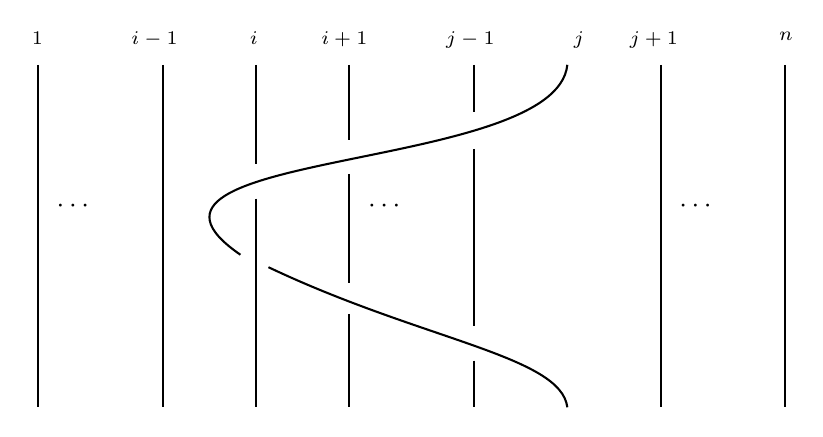
\begin{tikzpicture}[x=0.75pt,y=0.75pt,yscale=-1.5,xscale=1.5]
%uncomment if require: \path (0,877); %set diagram left start at 0, and has height of 877

%Straight Lines [id:da43079767492294996] 
\draw    (100,40) -- (100,150) ;
%Straight Lines [id:da8568972494568349] 
\draw    (140,40) -- (140,150) ;
%Straight Lines [id:da39499802412559726] 
\draw    (170,40) -- (170,72) ;
%Straight Lines [id:da06352980068118319] 
\draw    (200,40) -- (200,64) ;
%Straight Lines [id:da5832724793835432] 
\draw    (240,40) -- (240,55) ;
%Straight Lines [id:da9487132303393538] 
\draw    (300,40) -- (300,150) ;
%Straight Lines [id:da2547896303322166] 
\draw    (340,40) -- (340,150) ;
%Curve Lines [id:da9573368491042561] 
\draw    (270,40) .. controls (266.5,75) and (115.5,67) .. (165,101) ;
%Straight Lines [id:da3325229398873272] 
\draw    (170,83) -- (170,150) ;
%Curve Lines [id:da11849363606307461] 
\draw    (174,105) .. controls (223.5,128.5) and (268,133.5) .. (270,150) ;
%Straight Lines [id:da16906643654568176] 
\draw    (200,75) -- (200,110) ;
%Straight Lines [id:da11587080674469141] 
\draw    (200,120) -- (200,150) ;
%Straight Lines [id:da014801284669030856] 
\draw    (240,67) -- (240,124) ;
%Straight Lines [id:da15561552279853996] 
\draw    (240,135) -- (240,150) ;

% Text Node
\draw (105,82.4) node [anchor=north west][inner sep=0.75pt]    {$\cdots $};
% Text Node
\draw (205,82.4) node [anchor=north west][inner sep=0.75pt]    {$\cdots $};
% Text Node
\draw (305,82.4) node [anchor=north west][inner sep=0.75pt]    {$\cdots $};
% Text Node
\draw (97,28.4) node [anchor=north west][inner sep=0.75pt]  [font=\scriptsize]  {$1$};
% Text Node
\draw (129,28.4) node [anchor=north west][inner sep=0.75pt]  [font=\scriptsize]  {$i-1$};
% Text Node
\draw (167,28.4) node [anchor=north west][inner sep=0.75pt]  [font=\scriptsize]  {$i$};
% Text Node
\draw (190,28.4) node [anchor=north west][inner sep=0.75pt]  [font=\scriptsize]  {$i+1$};
% Text Node
\draw (230,28.4) node [anchor=north west][inner sep=0.75pt]  [font=\scriptsize]  {$j-1$};
% Text Node
\draw (271,28.4) node [anchor=north west][inner sep=0.75pt]  [font=\scriptsize]  {$j$};
% Text Node
\draw (289,28.4) node [anchor=north west][inner sep=0.75pt]  [font=\scriptsize]  {$j+1$};
% Text Node
\draw (337,28.4) node [anchor=north west][inner sep=0.75pt]  [font=\scriptsize]  {$n$};


\end{tikzpicture}

\end{center}
Nuevamente observemos como se ven estos grupos en los casos pequeños
\begin{eg}
    Es claro que $P_1=\{1\}$, para $P_2$ note que queremos trenzas no isotopicas a la identidad tales que su permutacion subyacente sea $(1,2)$, es claro que $A_{1,2}$ es una de ellas, pero recordemos que $B_2=\langle\sigma_1\rangle$, desde el diagrama nos podemos dar cuenta que $A_{1,2}=\sigma_1^2$, por lo que $P_2=\langle\sigma_2^2\rangle\cong2\Z$, ya que aplicar $\sigma_1$ un numero impar de veces siempre nos dara una trenza con permutacion subyacente $(2,1)$.
    \begin{center}
        

\tikzset{every picture/.style={line width=0.75pt}} %set default line width to 0.75pt        

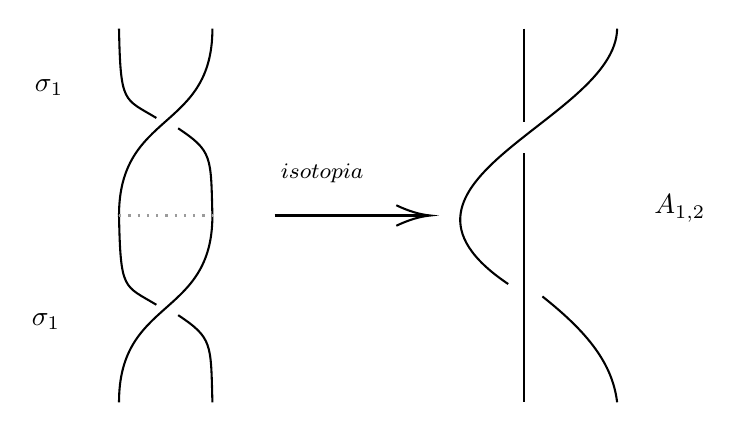
\begin{tikzpicture}[x=0.75pt,y=0.75pt,yscale=-1.5,xscale=1.5]
%uncomment if require: \path (0,877); %set diagram left start at 0, and has height of 877

%Curve Lines [id:da4483455906256475] 
\draw    (160,30) .. controls (160,63) and (130,56.33) .. (130,90) ;
%Curve Lines [id:da6523208333780345] 
\draw    (130,30) .. controls (130.5,54.33) and (131.5,52.33) .. (142,58.67) ;
%Curve Lines [id:da22555423095643323] 
\draw    (149,62) .. controls (160,69.33) and (159.5,71) .. (160,90) ;
%Curve Lines [id:da07435409788334091] 
\draw    (160,90) .. controls (160,123) and (130,116.33) .. (130,150) ;
%Curve Lines [id:da9140312091006156] 
\draw    (130,90) .. controls (130.5,114.33) and (131.5,112.33) .. (142,118.67) ;
%Curve Lines [id:da9801659584508721] 
\draw    (149,122) .. controls (160,129.33) and (159.5,131) .. (160,150) ;
%Straight Lines [id:da18469253279455966] 
\draw [color={rgb, 255:red, 155; green, 155; blue, 155 }  ,draw opacity=1 ] [dash pattern={on 0.84pt off 2.51pt}]  (130,90) -- (160,90) ;
%Straight Lines [id:da28298508987931226] 
\draw    (180,90) -- (228,90) ;
\draw [shift={(230,90)}, rotate = 180] [color={rgb, 255:red, 0; green, 0; blue, 0 }  ][line width=0.75]    (10.93,-3.29) .. controls (6.95,-1.4) and (3.31,-0.3) .. (0,0) .. controls (3.31,0.3) and (6.95,1.4) .. (10.93,3.29)   ;
%Curve Lines [id:da2405058001445326] 
\draw    (290,30) .. controls (289.5,59.5) and (206,79) .. (255,112) ;
%Straight Lines [id:da9678798921669155] 
\draw    (260,30) -- (260,60) ;
%Straight Lines [id:da9537331354112881] 
\draw    (260,70) -- (260,150) ;
%Curve Lines [id:da362550510769316] 
\draw    (266,116) .. controls (280.5,127.5) and (288.5,137.5) .. (290,150) ;

% Text Node
\draw (102,45.4) node [anchor=north west][inner sep=0.75pt]    {$\sigma _{1}$};
% Text Node
\draw (101,120.4) node [anchor=north west][inner sep=0.75pt]    {$\sigma _{1}$};
% Text Node
\draw (181,72.4) node [anchor=north west][inner sep=0.75pt]  [font=\footnotesize]  {$isotopia$};
% Text Node
\draw (301,82.4) node [anchor=north west][inner sep=0.75pt]    {$A_{1,2}$};


\end{tikzpicture}
    \end{center}
\end{eg}
De la misma manera en que la inclusión $i:B_n\to B_{n+1}$ añadía una cuerda al diagrama que no interactuaba con otras a la derecha del todo, se puede considerar $i|_{P_n}$,de manera similar podemos pensar en una función que elimine alguna cuerda. Note que esa nocion de eliminar no es conveniente trabajarla directamente en $B_n$ ya que los puntos finales e iniciales de cada cuerda no son los mismos, por lo que podríamos tener algún problema al definirlo, pero en $P_n$ no tendríamos por que preocuparnos
\begin{definition}
    Definimos el \textit{homomorfismo de olvido} $f_n:P_n\to P_{n-1}$ tal que a una trenza geométrica en $P_n$, se elimina la trenza con puntos $(n,0,0)$ y $(n,0,1)$ iniciales y finales respectivamente.
\end{definition}
La función esta bien definida en clases de isotopia ya que dadas dos trenzas en $P_n$ isotopicas, al eliminar la misma cuerda la isotopia sigue actuando igual sobre las trenzas en $P_{n-1},$ ya que en cada paso es simplemente olvidar la deformación sobre la n-esima cuerda, que sea homomorfismo de grupos es inmediato de la definición de multiplicación de trenzas ya que es solo la concatenación de diagramas y como los puntos finales e iniciales de cada cuerda son el mismo se sigue manteniendo el hecho de que sean trenzas. En vistas de esto. Con esto de manera similar a lo hecho con $\pi$ sera util en un futuro considerar el siguiente subgrupo.
\begin{definition}
    Para $n\geq 2$ definimos
    $$U_n=\ker f_n.$$
\end{definition}
De manera inmediata no se ve la razon particular de definir este subgrupo, mas sera útil posteriormente para estudiar propiedades algebraicas.
\begin{eg}
    Dada la trenza $A_{2,5}$, por el diagrama es claro que $f_5(A_{2,5})=1_4$, asi $A_{2,5}\in U_5$, en general es facil notar del diagrama general que $A_{i,n}\in U_n$ para $1\leq i<n$.
\end{eg}
Retomaremos la discusión de estos objetos en proximas secciones donde con las equivalencias ya tengamos mas herramientas, ahora volvamos a la nocion de los espacios de configuración, que si bien esta primera nocion no es una equivalencia directa con el grupo $B_n$ nos abre el camino para la misma
\begin{theorem}
    Para $M=\R^2$ tenemos que $\pi_1(\mathcal{F}_n(M))\cong P_n.$
\end{theorem}
\begin{proof}
    La idea a seguir sera enviar las trenzas puras geométricas a los posibles lazos. Sea $b\subset \R^2\times I$, definamos la imagen de $b$ como el camino $I\to \mathcal{F}_n(\R^2)$, donde $t\mapsto(u_1(t),\ldots,u_n(t))$, donde el camino tiene que cumplir que la $i-$esima cuerda de $b$ intersecta a el plano $\R^2\times\{t\}$ en el punto $(u_i(t),t)$ para todo $i=1,\ldots,n.$ Con esto estamos aprovechando el hecho de que en cada plano hay $n$ puntos diferentes. Asi note que esto nos da un camino que inicia y termina en el punto $q_n=((1,0),\ldots,(n,0))$, esto debido a que es una trenza pura. Para hacer la otra asignación un camino $(\alpha_1,\ldots,\alpha_n):I\to \mathcal{F}_n(\R^2)$ con punto inicial y final $q_n$. Podemos considerar el siguiente conjunto
    $$\bigcup_{i=1}^n\bigcup_{t\in I}(\alpha_i(t),t).$$
    Note que como cada $\alpha_i(t)$ es un camino continuo y $t\in I$ estamos creando cada cuerda a partir de este camino, y al ser elementos del espacio de configuración cumplimos la condición de ser disjuntos. Estas construcciones son inversas la una de la otra y dan una correspondencia entre lazos y trenzas geométricas puras, de la forma $P_n=\pi_1(\mathcal{F}_n(\R^2),q_n).$  
\end{proof}

\textcolor{blue}{Continuar con no ordenados luego.}